\chapter{Heuristics}\label{chap:heuristics}

\begin{quotation}
      ``It is not the strongest of the species that survives. It is also not the most intelligent that survives. It is the one that is the most adaptable to change.''
\end{quotation}
\begin{flushright}
      - Charles Darwin
\end{flushright}

Many different techniques have been used to train \acp{FFNN}~\cite{ref:kingma:2014}. Finding the best technique to use to train a \acs{FFNN} has been shown to be problem dependent in many cases~\cite{ref:kheiri:2017}. Every technique has its characteristics, constraints, advantages and disadvantages. At the time of writing, the majority of work that is published around the training of \acp{FFNN}, involves the use of gradient-based techniques~\cite{ref:nel:2021}. Gradient-based techniques are not without flaws and can, for example, yield slow convergence or get trapped in local optima~\cite{ref:mingguang:2009}. Other techniques have also been used to successfully train \acp{FFNN}, including \acp{MH} such as \acf{PSO}~\cite{ref:rakitianskaia:2012, ref:vanwyk:2014}, \acf{DE}~\cite{ref:espinal:2011} and \acfp{GA}~\cite{ref:gupta:1999}.

Chapter~\ref{chap:anns} briefly introduced the reader to the concept of \index{heuristic}\index{heuristic}heuristics and \acfp{MH}s. This chapter presents more detailed background information on various different \index{heuristic}heuristics that have been used to train \acp{FFNN}. Broadly speaking, this chapter focuses on two different groups of \index{heuristic}heuristics, including classical gradient-based approaches and population-based \acp{MH}. Each technique is presented and discussed in detail. Pseudo-code algorithms are provided for each technique and discussions follow on advantages, disadvantages, capabilities and limitations. The remainder of this chapter is structured as follows:

\begin{itemize}
      \item \textbf{Section~\ref{sec:heuristics:optimisation}} provides a brief review of optimisation. It is shown that training of \acp{FFNN} is an optimisation problem.

      \item \textbf{Section~\ref{sec:heuristics:what_is_a_heuristic}} provides background information on the origins and definition of the term \index{heuristic}\textit{heuristic}. It is shown that \index{heuristic}heuristics are a class of algorithms that are used to solve optimisation problems.

      \item \textbf{Section~\ref{sec:heuristics:gd}} presents seven low-level, gradient-based \index{heuristic}heuristics, including \acf{SGD}, \acf{Momentum}, \acf{NAG}, \acf{Adagrad}, \acf{RMSProp}, \acf{Adadelta} and \acf{Adam}.

      \item \textbf{Section~\ref{sec:heuristics:mh}} presents three different population-based \acp{MH}, including \acf{PSO}, \acf{DE} and \acfp{GA}.

      \item \textbf{Section~\ref{sec:heuristics:summary}} provides a brief summary of the chapter.
\end{itemize}

\section{Optimisation}\label{sec:heuristics:optimisation}

Optimisation is the task of finding a solution to a given problem that is better than alternative solutions. Better stated by \citeauthor{ref:oldewage:2017}~\cite{ref:oldewage:2017}, optimisation is the task of finding values for a set of variables such that some measure of optimality is satisfied given a set of constraints. \citeauthor{ref:engelbrecht:2007}~\cite{ref:engelbrecht:2007} breaks optimisations problems down into three components:

\begin{itemize}
      \item An \textbf{objective function}: Represents the quantity to be optimised and is used as the ``measure of optimality''. Optimisation can be defined in terms of the minimisation or maximisation of the objective function $f$.

      \item A \textbf{set of unknowns or independent variables}: Affects the outcome of the objective function $f$ and is denoted as $x$. $f(x)$ is thus the quantification of the objective function over the unknowns, represented by $x$. Note that $x$ could be a scalar value, a vector or a matrix and notation is left out for simplicity.

      \item A \textbf{set of constraints}: Restrict and limit the values that can be assigned to the unknowns, represented by $x$. Optimisation problems that must adhere to a set of constraints are referred to as \acfp{CSP}.
\end{itemize}

Optimisation problems come in a wide variety, and can be defined in terms of the number of variables used (uni- vs. multivariate), the number of objective functions used (single- vs. multi-objective), the degree of linearity (linear vs. quadratic/polynomial), the number of optima (uni- vs. multi-modal), the nature of the environment (static vs. dynamic), the types of variables used (separable vs. inseparable, discrete vs. continuous) and the set of constraints that the solution must adhere to (constrained vs unconstrained).

Optima can be defined as \textit{local} or \textit{global} optima. Local optima is the best optimisation of $f(x)$ in a neighbourhood of solutions, while the global optima is the best optimisation of $f(x)$ over all solutions in the solution space.

As stated in Chapter~\ref{chap:anns}, the training of an \acp{FFNN} is a particular type of optimisation problem, where the goal is to find the configuration of \textit{weights}, such that the \acs{FFNN} yields output that minimises some loss function. The mechanism by which the optimal weights for a \acs{FFNN} is sought out, is executed by an \index{optimisation algorithm}optimisation algorithm known as a \index{heuristic}heuristic.

\section{What is a heuristic?}\label{sec:heuristics:what_is_a_heuristic}

The term \textit{heuristic} comes from the Latin word \textit{heuristicus} which means ``to find out or discover''.~\citeauthor{ref:romanycia:1985}~\cite{ref:romanycia:1985} provide a complete study on the history and origins of the term \index{heuristic}\textit{heuristic}. From their research, a proposal is made to define \index{heuristic}heuristics in the context of \acf{AI}, as any device, be it a program, rule, piece of knowledge, which is added to a problem-solving system, in expectation that, on average, the performance will improve.

In the context of this dissertation, a \index{heuristic}heuristic refers to an algorithmic search technique that serves as a guide to a search process where good solutions to a optimisation problem is being sought out. Different \index{heuristic}heuristics make use of different information during the search process~\cite{ref:kheiri:2017}. During training of \acp{FFNN}, \index{heuristic}heuristics such as gradient-based \index{heuristic}heuristics make use of the derivatives obtained by evaluating the \acs{FFNN}. It can thus be said that gradient-based \index{heuristic}heuristics make use of information directly from the \textit{search space}. On the contrary, \index{heuristic}heuristics such as \acp{MH} make use of meta-information obtained as a result of evaluating the \acs{FFNN}~\cite{ref:blum:2003}. The meta-information that \acp{MH} make use of could include ranked-performance of a population of candidate solutions, referred to as \textit{entities}. \index{meta-heuristic}Meta-heuristics are useful when there is imperfect information about the search space~\cite{ref:bianchi:2009}, and are generally less problem-specific than other classes of \index{heuristic}heuristics~\cite{ref:blum:2003}. This dissertation takes a particular interest in gradient-based \index{heuristic}heuristics and \acp{MH}.


\section{Gradient-Based Heuristics}\label{sec:heuristics:gd}

Gradient-based \index{heuristic}heuristics are optimisation techniques that make use of derivates obtained from evaluating the model being optimised. Specifically, in the context of a minimisation problem, these techniques are called \acf{GD} heuristics as they \textit{minimise} some loss function. \Acs{GD} is generally attributed to Cauchy~\cite{ref:lemarechal:2012}, who first suggested it in 1847. In 1907 Hadamard~\cite{ref:hadamard:1908} independently proposed a similar method.

Although gradient-based \index{heuristic}heuristics where not the first \index{heuristic}heuristics used to train \acp{FFNN}
\cite{ref:engelbrecht:2007}, they are certainly the most widely used. Gradient-based heuristics have become increasingly popular partly due to their simplicity and low computational overhead compared to other \index{heuristic}heuristics such as \acp{MH} and other second-order derivative methods such as Newtons' method. There are many variants of gradient-based \index{heuristic}heuristics, however, they all fundamentally apply the same generic \acf{GD} framework called \acf{BP}.

\subsection{Backpropagation}\label{sec:heuristics:gd:backpropagation}

Chapter~\ref{chap:anns} introduced \index {supervised learning}supervised learning and presented a number of loss functions. In the context of supervised learning, loss functions produce a scalar value $\epsilon$, that represents the error between the output of the \acs{FFNN} and the desired output. When using \acs{GD} to train \acp{FFNN}, the \index{loss function}loss function is used to adjust the weights of the \acs{FFNN} in order to minimise the error~\cite{ref:engelbrecht:2007}.~\citeauthor{ref:engelbrecht:2007}~\cite{ref:engelbrecht:2007} states that training of \acp{FFNN} using \acs{GD}, is done by calculating the gradient of $\epsilon$ in \textit{weight-space}, and then moving the weight vector along the negative gradient. An illustration of \acs{GD} is given in Figure~\ref{fig:heuristics:gd:gd_illustration}.

\begin{figure}[htbp]
      \centering
      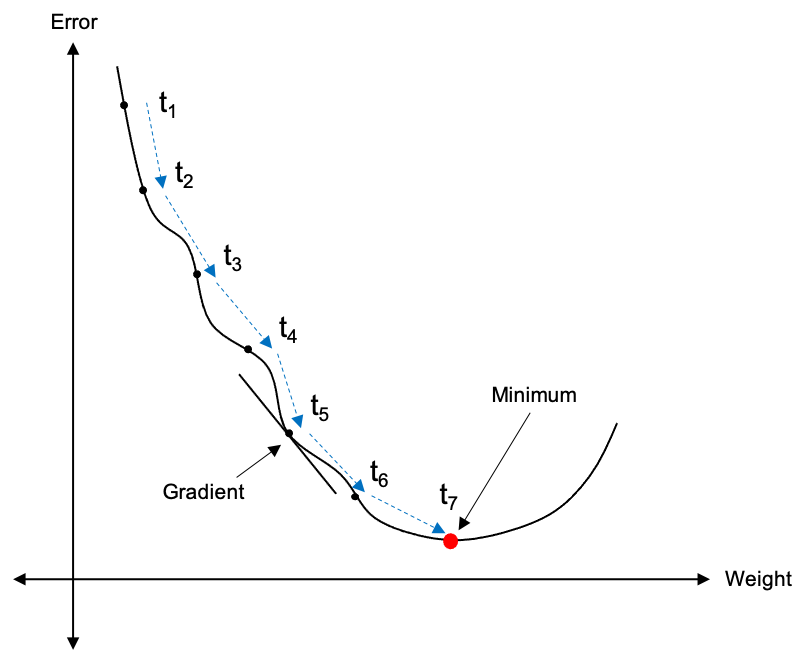
\includegraphics[width=0.75\textwidth]{images/gradient_descent.pdf}
      \caption{An illustration of \acf{GD} over various time steps showing the minimisation of the error with regards to weight value.}
      \label{fig:heuristics:gd:gd_illustration}
\end{figure}

In the context of training \textit{shallow} \acp{FFNN} using \index{supervised learning}supervised learning, the error signal is propagated backwards in the network from the output layer, through the hidden layer to the input layer, updating the weights at the output and hidden layers. The algorithm that propagates the error signal backwards is known as \acf{BP}. \Acs{BP} was popularised by~\citeauthor{ref:werbos:1994}~\cite{ref:werbos:1994}.~\citeauthor{ref:nel:2021}~\cite{ref:nel:2021} states that \acs{BP} provides a procedure for updating the network weights, layer by layer, by evaluating the derivatives of the error function $\mathcal{E}$, with respect to the weights at each layer.~\citeauthor{ref:engelbrecht:2007}~\cite{ref:engelbrecht:2007} describes the \acs{BP} process in two steps:

\begin{itemize}
      \item \textbf{Feedforward Pass}: During this phase the output values of the \acs{FFNN} is calculated for each training pattern.

      \item \textbf{Backward Propagation}: During this phase the error signal is propagated backwards from the output layer, through the hidden layer, to the input layer of the \acs{FFNN}. Weights at the output and hidden layers are then adjusted as functions of the backpropagated error signal.
\end{itemize}

The update step for \acs{GD} by means of \acs{BP} can be formulated as is shown in Equations~\eqref{eq:heuristics:gd:update_step_part_1} to \eqref{eq:heuristics:gd:update_step_part_4}. The general weight update step is given as

\begin{equation}
      \label{eq:heuristics:gd:update_step_part_1}
      w_{i}(t) = w_{i}(t-1) + \Delta w_{i}(t)
\end{equation}

where $w_{i}$ is the weight value at index $i$, $t$ is the time step, $\Delta w_{i}(t)$ is the weight update vector at index $i$ and time step $t$. The delta weight term $\Delta w_{i}(t)$, is given as

\begin{equation}
      \label{eq:heuristics:gd:update_step_part_2}
      \Delta w_{i}(t) = -\eta\frac{\partial \epsilon}{\partial w_{i}}
\end{equation}

where $\eta$ is the learning rate and $\frac{\partial \epsilon}{\partial w_{i}}$ is the \textit{gradient} of the error, as a result of a loss function $\mathcal{E}$, relative to the weight at index $i$. The learning rate controls the step-size that is taken in the direction of the negative gradient at each time step. Assuming the use of \acs{SSE} as the loss function, the partial derivative of $\epsilon$, relative to the weight $w$, at index $i$, is given as

\begin{equation}
      \label{eq:heuristics:gd:update_step_part_3}
      \frac{\partial \epsilon}{\partial w_{i}} = -2(t_{p} - o_{p})\frac{\partial f}{\partial net_{p}}z_{i,p}
\end{equation}

where $t_{p}$ refers to the target value for pattern $p$, $o_{p}$ refers to the output value for pattern $p$, $f$ refers to the \index{activation function}activation function, $net_{p}$ refers to the \index{net input signal}net input signal for pattern $p$, and $z_{i,p}$ refers to the input value at index $i$ for pattern $p$.

Finally, assuming the use of the \index{sigmoid}sigmoid activation function, the partial derivative of the activation function, relative to the net input signal is given as

\begin{equation}
      \label{eq:heuristics:gd:update_step_part_4}
      \frac{\partial f}{\partial net_{p}} = o_p(1 - o_{p})
\end{equation}

Again, assuming the use of \acs{SSE} as the loss function, the pseudo-code implementation for the generic \acs{GD} algorithm is taken from~\citeauthor{ref:engelbrecht:2007}~\cite{ref:engelbrecht:2007} and is presented in Algorithm~\ref{algo:heuristics:gd:gd} below.

\begin{algorithm}[htb]
      \caption{The pseudo-code algorithm for the generic \acf{GD} heuristic.}
      \label{algo:heuristics:gd:gd}
      \begin{algorithmic}
            \State Initialise the \acs{FFNN} weights and biases, the learning rate $\eta$ and the time step/epoch $T=0$;
            \While{stopping conditions are not met}
            \State Let $\epsilon_{T} = 0$;
            \For{each training pattern p}
            \State Calculate the output of the hidden and output layers (feedforward);
            \State Compute the error signals of the hidden and output layers;
            \State Adjust the weights of the output and hidden layers (backpropagate);
            \State $\epsilon_{T}$ += $[\epsilon_{T_{p}} = \sum^{K}_{k=1}(t_{k,p} - o_{k,p})^{2}]$;
            \EndFor
            \State $T += 1$;
            \EndWhile
      \end{algorithmic}
\end{algorithm}

A simplified notation is proposed from which the gradient-based heuristics can be compared. Consider a simplification of the update-step for \acs{SGD} as presented in Equations~\eqref{eq:heuristics:gd:update_step_part_1} and~\eqref{eq:heuristics:gd:update_step_part_2} where $\frac{\partial \epsilon}{\partial w_{i}}$ is simply represented as the gradient term $g$, resulting in a simplified weight update step and is given as

\begin{equation}
      \label{eq:heuristics:gd:sgd}
      \begin{split}
            \boldsymbol{w} = \boldsymbol{w} - \eta \boldsymbol{g}
      \end{split}
\end{equation}

where $\boldsymbol{w}$ refers to the weight vector, $\eta$ refers to the learning rate as before and $\boldsymbol{g}$ refers to the gradient of the error function relative to weight vector. Note that some subscripts related to layers, indices, time steps and training patterns are omitted for convenience.

\subsection{Stochastic vs. Batch Training}\label{sec:heuristics:gd:sgd}

This section shines light on the algorithmic implementation of \acs{BP} with specific context to stochastic and batch training. The implementation of \acs{GD} using stochastic training is referred to as \acf{SGD}.

\acs{SGD} was one of the first widely used heuristics to train \acs{FFNN}, however, it is not without flaws. With stochastic training, only one training pattern is presented at each iteration/epoch. As such, weight updates are done with high variance and noise~\cite{ref:ruder:2016}. An illustration of the fluctuations caused by \acs{SGD} during training is given in Figure~\ref{fig:heuristics:gd:sgd}.

\begin{figure}[htbp]
      \centering
      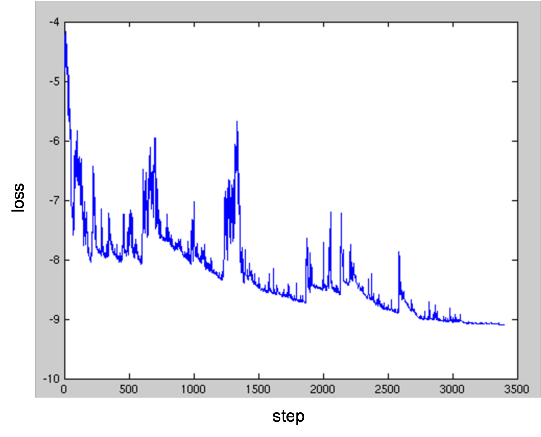
\includegraphics[width=0.8\textwidth]{images/sgd.pdf}
      \caption{An illustration of \acf{SGD} fluctuations during training as taken from~\cite{ref:sgd:2006}.}
      \label{fig:heuristics:gd:sgd}
\end{figure}

With batch training, all the training patterns are presented at once and the \acs{FFNN} converges to the global minimum of the loss function w.r.t $\boldsymbol{w}$ (assuming the loss function is convex). However, this is computationally expensive and impractical to implement in many situations. While \acs{SGD} is able to jump out of local minima into new, potentially better local minima~\cite{ref:ruder:2016}, \acs{SGD} complicates convergence to the minima as \acs{SGD} can potentially keep overshooting better minima. By slowly decreasing the learning rate $\eta$ during training, the same convergence behaviour is achieved as with batch training.

A compromise is to make use of mini-batches of training patterns, where a small number of training patterns are presented to the \acs{FFNN} at once. This is referred to as \textit{mini-batch} training. Input patterns from mini-batches are approximations of the total population of training patterns. According to~\citeauthor{ref:ruder:2016}~\cite{ref:ruder:2016} this has two main advantages:

\begin{itemize}
      \item Mini-batch training reduces the high variance of weight updates as observed for \acs{SGD}, which leads to better convergence.

      \item Mini-batch training allows for the implementation of \acs{GD} using highly optimised matrix operations, common to the state-of-the-art \acs{ML} libraries used today.
\end{itemize}

In the context of this dissertation, the implementation of \acs{SGD} refers to the mini-batch training implementation of \acs{GD}. Although mini-batch training does provide a compromise between stochastic and batch training, there are still a number of challenges faced by mini-batch training. These include:

\begin{itemize}
      \item The appropriate value to use for the learning rate $\eta$, is difficult to determine and is often problem-specific. A learning rate that is too small causes premature exploitation, leading to slow and bad convergence. On the contrary, a learning rate that is too high may lead to bad learning outcomes as the heuristic keeps overshooting good minima.

      \item Learning rate schedules~\cite{ref:robbins:1951} can be introduced to dynamically change the learning rate throughout the training process, however, these schedules and their parameters have to be defined a priori and are often problem specific~\cite{ref:darken:1992}.

      \item The learning rate that has been introduced so far is applied to all elements of the weight update vector. If the training data is sparse and the features have varying frequencies, an equal update to all weight elements is inefficient. Larger weight updates are required for less frequently occurring features. Inefficient updates of all elements in the weight vectors contribute to the credit assignment problem~\cite{ref:rumelhart:1986}, common to \acs{GD} variants.

      \item It is difficult to avoid getting trapped in local minima, especially for highly non-convex loss functions used for training \acp{FFNN}. \citeauthor{ref:dauphin:2014}~\cite{ref:dauphin:2014} mentions the role of saddle points in getting trapped in local minima. Saddle points are points at which one dimensions slopes upwards, while another dimension slopes downwards. \citeauthor{ref:ruder:2016}~\cite{ref:ruder:2016} mentions that these saddle points are usually surrounded by plateaus of the same error, leading to gradients that are close to zero in all dimensions.
\end{itemize}

Alternative variants have been proposed that lead to better control over the convergence characteristics caused by \acs{GD}. The first of these \acs{GD} variants include \acs{Momentum}.

\subsection{Momentum}\label{sec:heuristics:gd:momentum}

Research shows that \acs{SGD} has difficulty navigating ravines~\cite{ref:sutton:1986}. Ravines are areas where the surface curves much more steeply in one dimension than in another. These ravines are common around local minima. As such, \acs{SGD} is shown to oscillate across the slopes of the ravine while only making minor progress towards the local minima.

\Acs{Momentum} ~\cite{ref:qian:1999} is a variant of \acs{SGD} that helps accelerate \acs{SGD} in the relevant direction, dampening oscillations.~\citeauthor{ref:ruder:2016}~\cite{ref:ruder:2016} mentions that this is done by adding a fraction $\alpha$, of the weight update vector of the previous time step to the current weight update vector. An illustration of \acs{SGD} with and without momentum is given in Figure~\ref{fig:heuristics:gd:sgd_with_and_without_momentum}.

\begin{figure}[htbp]
      \centering
      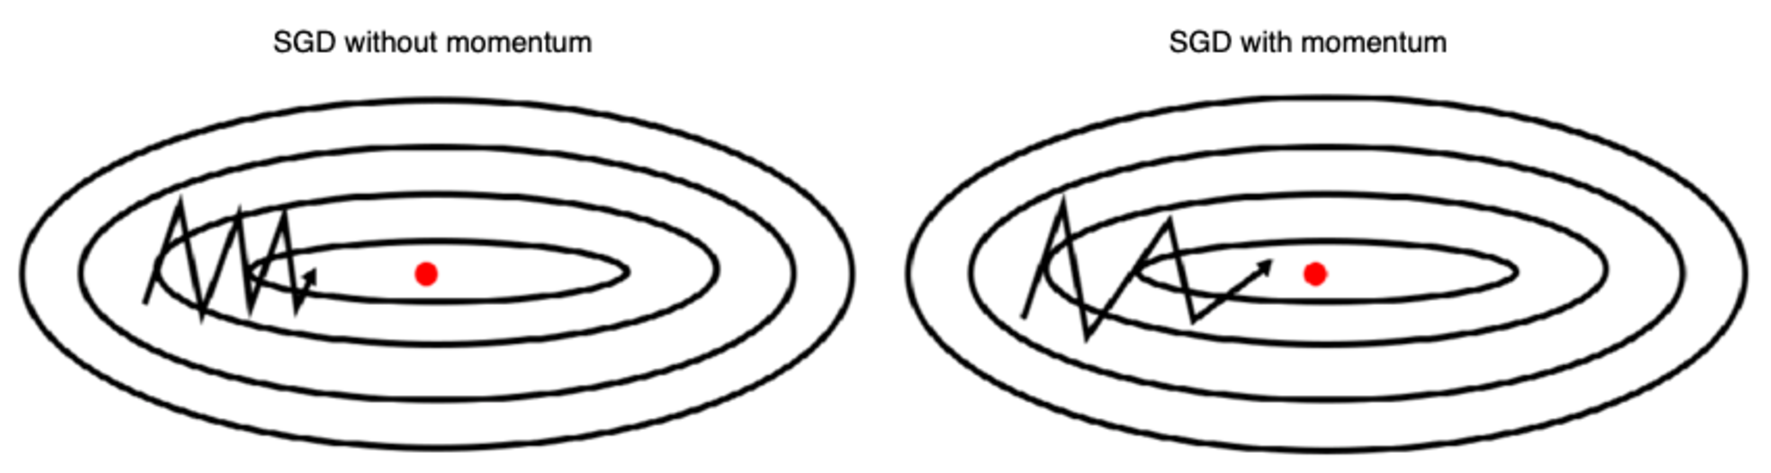
\includegraphics[width=0.99\textwidth]{images/sgd_with_and_without_momentum.pdf}
      \caption{An illustration of \acf{SGD} with and without momentum taken from~\cite{ref:du:2019}.}
      \label{fig:heuristics:gd:sgd_with_and_without_momentum}
\end{figure}

The accumulation of momentum is presented in Equation~\eqref{eq:heuristics:gd:momentum_part_1}, while the update step is then amended in Equation~\eqref{eq:heuristics:gd:momentum_part_2}.

\begin{equation}
      \label{eq:heuristics:gd:momentum_part_1}
      \begin{split}
            \boldsymbol{v} = \alpha \boldsymbol{v} - \eta \boldsymbol{g}
      \end{split}
\end{equation}

\begin{equation}
      \label{eq:heuristics:gd:momentum_part_2}
      \begin{split}
            \boldsymbol{w} = \boldsymbol{w} + \boldsymbol{v}
      \end{split}
\end{equation}

By redefining the \acs{SGD} update steps as shown above in Equations~\eqref{eq:heuristics:gd:momentum_part_1} and~\eqref{eq:heuristics:gd:momentum_part_2}, the \acs{Momentum} heuristic allows for the increase of momentum for dimensions whose gradients point in the same direction, while simultaneously reducing momentum for dimensions whose gradients change direction, leading to faster convergence and less oscillation. The momentum term $\alpha$ is usually set to 0.9~\cite{ref:engelbrecht:2007, ref:ruder:2016}.

\subsection{Nesterov Accelerated Gradients}\label{sec:heuristics:nag}

\Acf{NAG} is a variant of the \acs{Momentum} heuristic developed by~\citeauthor{ref:sutskever:2013}~\cite{ref:sutskever:2013} and is inspired by~\citeauthor{ref:nesterov:1983}'s~\cite{ref:nesterov:1983} work on optimising convex functions. \acs{NAG} provides an improvement to the momentum accumulation term by providing a look-ahead term that better refines the weight update step.

In the \acs{NAG} heuristic, the gradient is not calculated w.r.t the current weights, but rather w.r.t the approximate future positions of the weights~\cite{ref:sutskever:2013, ref:ruder:2016}. An illustration of the weight update vector using \acs{NAG} is taken from Geoffrey Hinton's lecture on mini-batch \acs{GD}~\cite{ref:hinton:2012} and is presented in Figure~\ref{fig:heuristics:gd:nag} below.

\begin{figure}[htbp]
      \centering
      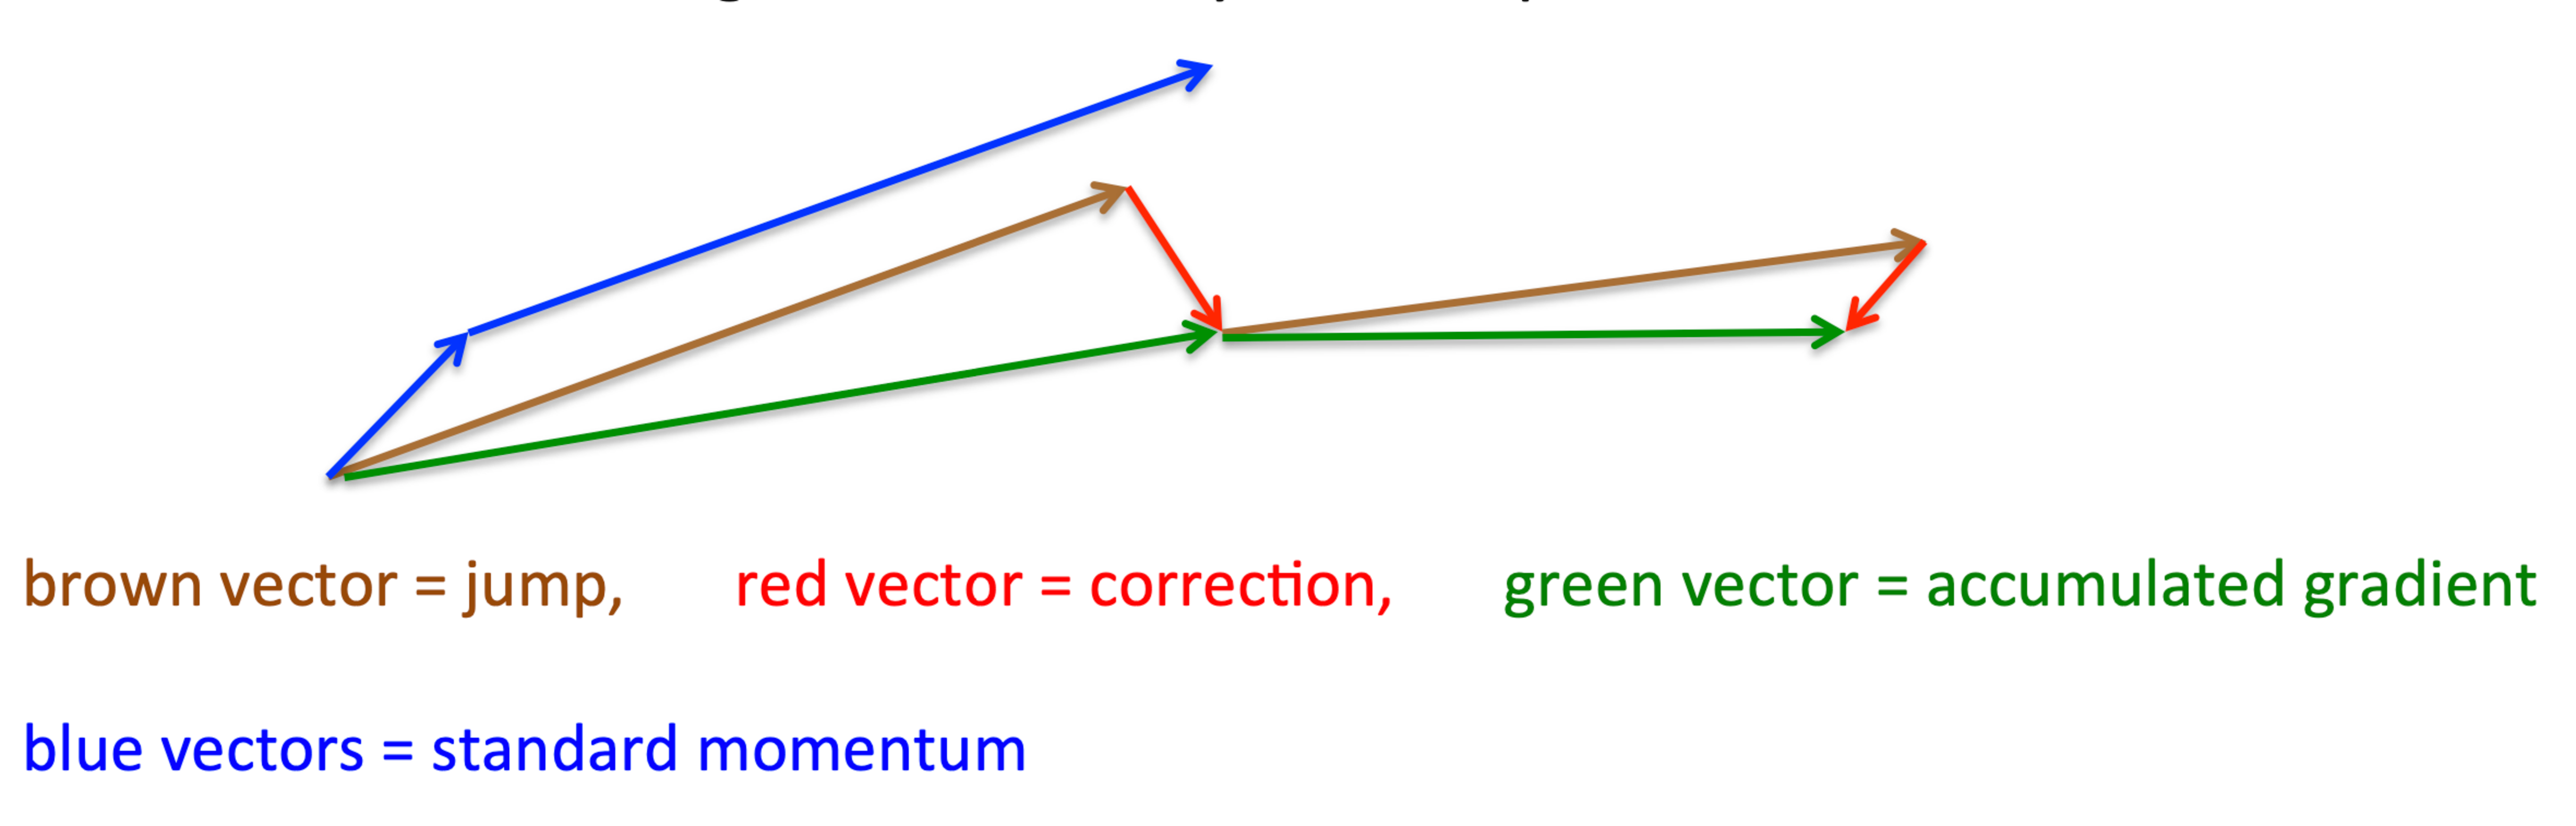
\includegraphics[width=0.95\textwidth]{images/nag.pdf}
      \caption{An illustration of the weight update vector for \acf{NAG} taken from~\cite{ref:hinton:2012}.}
      \label{fig:heuristics:gd:nag}
\end{figure}

The difference in the update step for \acs{Momentum} and the update step for \acs{NAG} as developed by~\citeauthor{ref:sutskever:2013}~\cite{ref:sutskever:2013} is described by~\citeauthor{ref:ruder:2016}~\cite{ref:ruder:2016} as follows. \acs{Momentum} first calculates the current gradient, represented by the small \textcolor{blue}{blue} vector in Figure~\ref{fig:heuristics:gd:nag} and then takes a large step in the direction of the updated accumulated gradient, presented by the big \textcolor{blue}{blue} vector. In contrast, \acs{NAG} first takes a big step in the direction of the previous accumulated gradient presented by the \textcolor{brown}{brown} vector. At this point the gradient is measured and \acs{NAG} makes a correction represented by the \textcolor{red}{red} vector. The complete update step is represented by the green vector. By anticipating approximate future positions of the weights, the weight update step as defined by \acs{NAG} controls the optimisation process from going too fast and results in increased responsiveness~\cite{ref:bengio:2013}. Along with the same velocity update step for \acs{Momentum}, as presented in Equation~\eqref{eq:heuristics:gd:momentum_part_1}, the \acs{NAG} weight update step is given as

\begin{equation}
      \label{eq:heuristics:gd:nag_part_2}
      \begin{split}
            \boldsymbol{w} = \boldsymbol{w} + \alpha \boldsymbol{v} - \eta \boldsymbol{g}
      \end{split}
\end{equation}


\subsection{Adaptive Gradients}\label{sec:heuristics:adagrad}

\Acf{Adagrad} is an adaptation of \acs{SGD} that implements a learning rate for every element in the weight vector and is developed by \citeauthor{ref:duchi:2011}~\cite{ref:duchi:2011}.~\citeauthor{ref:ruder:2016}~\cite{ref:ruder:2016} mentions that \acs{Adagrad} adapts the learning rate to the elements of the weight vector, by  performing small updates (i.e. low learning rates) for weights associated with frequently occurring features and larger updates (i.e. high learning rates) for weights associated with infrequent features. For this reason, \acs{Adagrad} is well suited for dealing with situations where training data is sparse.

In the \acs{GD} variants presented thus far, the weight updates have been applied by making use of the same learning rate $\eta$, for all elements of the weight update vector. \Acs{Adagrad} uses a different learning rate for every weight element $w_{i}$, at every time step $t$. The weight update step for \acs{Adagrad} is given as

\begin{equation}
      \label{eq:heuristics:gd:adagrad_part_1}
      \begin{split}
            w_{t+1,i} = w_{t,i} - \frac{\eta}{\sqrt{G_{t,ii} + \epsilon}}.g_{t,i}
      \end{split}
\end{equation}

where $w_{i}$ is the $i$-th element of the weight vector, $G_{t,ii} \in \mathbb{R}^{d \times d}$ is a diagonal matrix where each diagonal element $i,i$, is the sum of the squared gradients w.r.t. $w_{i}$, up to time step $t$ and $\epsilon$ is a smoothing term that avoids division by zero and is set to an insignificant value such as $1 \times 10^{-8}$. Since $\boldsymbol{G_{t}}$ contains the sum of the squares of the gradients along its diagonal, the weight update step can be vectorised and updated using the matrix-vector product, represented by $\odot$, between $G_{t,i}$ and $g_{t,i}$. The simplified update step as implemented by \acs{Adagrad} is given as

\begin{equation}
      \label{eq:heuristics:gd:adagrad_part_2}
      \begin{split}
            w_{t+1} = w_{t} - \frac{\eta}{\sqrt{G_{t,i} + \epsilon}} \odot g_{t,i}
      \end{split}
\end{equation}

\Ac{Adagrad}'s main benefit is that it does not require manual tuning of the learning rate $\eta$. However, a problem with \acs{Adagrad} is in the accumulation of squared gradients in the denominator, represented by $\boldsymbol{G_{t}}$. Since every term that is added is positive, $\boldsymbol{G_{t}}$ keeps growing, leading to a situation where the learning rate shrinks to the point that the heuristic is no longer able to learn.

\subsection{Adaptive Learning Rate}\label{sec:heuristics:adadelta}

\citeauthor{ref:zeiler:2012}~\cite{ref:zeiler:2012} presents \acs{Adadelta}, an improvement of \acs{Adagrad} that eliminates the accumulation of squared gradients in the denominator.~\citeauthor{ref:ruder:2016}~\cite{ref:ruder:2016} mentions that instead of accumulating all past squared gradients as in the case of \acs{Adagrad}, \acs{Adadelta} restricts the window of accumulation to a window with a fixed size $W$. However, storing $W$ previous squared gradients is very inefficient. Instead, the accumulation of gradients over $W$ steps is defined recursively as a decaying average of all past squared gradients. The moving average of squared gradients at time step $t$, denoted by $E[\boldsymbol{g}^{2}]_{t}$  depends on a fraction $\alpha$ of the previous average of squared gradients and the current gradient, similar to the update step for \acs{Momentum}. Also similar to \acs{Momentum}, $\alpha$ is set to 0.9. The update step for $E[\boldsymbol{g}^{2}]_{t}$ is given as

\begin{equation}
      \label{eq:heuristics:gd:adadelta_part_1}
      \begin{split}
            E[\boldsymbol{g}^{2}]_{t} = \alpha E[\boldsymbol{g}^{2}]_{t - 1} + (1 - \alpha)\boldsymbol{g}_{t}^{2}
      \end{split}
\end{equation}

To illustrate the difference between \acs{Adagrad} and \acs{Adadelta}, the \acs{SGD} weight update step for \acs{Adagrad}, as presented in~\eqref{eq:heuristics:gd:adagrad_part_2} is rewritten such that the diagonal matrix $\boldsymbol{G_{t}}$, is replaced with the moving average of squared gradients and is given as

\begin{equation}
      \label{eq:heuristics:gd:adadelta_part_2}
      \begin{split}
            \boldsymbol{w}_{t+1} = \boldsymbol{w}_{t} - \frac{\eta}{\sqrt{E[\boldsymbol{g}^{2}]_{t} + \epsilon}} \boldsymbol{g}_{t}
      \end{split}
\end{equation}

Since the denominator is the \acf{RMS} error criterion of the gradient, the criteria short-hand notation is used and is given as

\begin{equation}
      \label{eq:heuristics:gd:adadelta_part_3}
      \begin{split}
            \boldsymbol{w}_{t+1} = \boldsymbol{w}_{t} - \frac{\eta}{RMS[\boldsymbol{g}]_{t}} \boldsymbol{g}_{t}
      \end{split}
\end{equation}

~\citeauthor{ref:zeiler:2012}~\cite{ref:zeiler:2012} noted that the units of the update step as presented in Equation~\eqref{eq:heuristics:gd:adadelta_part_3} do not match. The weight update vector should have the same hypothetical units as the weight vector. To fix the aforementioned problem, another exponentially decaying average is defined in terms of squared weight updates and is given as

\begin{equation}
      \label{eq:heuristics:gd:adadelta_part_4}
      \begin{split}
            E[\Delta \boldsymbol{w}^{2}]_{t} = \alpha E[\Delta \boldsymbol{w}^{2}]_{t - 1} + (1 - \alpha)\Delta \boldsymbol{w}_{t}^{2}
      \end{split}
\end{equation}

The \acf{RMS} error of weight updates is given as

\begin{equation}
      \label{eq:heuristics:gd:adadelta_part_5}
      \begin{split}
            RMS[\Delta \boldsymbol{w}]_{t} = \sqrt{E[\Delta \boldsymbol{w}^{2}]_{t} + \epsilon}
      \end{split}
\end{equation}

Note that $RMS[\Delta \boldsymbol{w}]_{t}$ is unknown at time step $t$. $RMS[\Delta \boldsymbol{w}]_{t}$ is approximated with the \acf{RMS} of weight updates until the previous time step. The learning rate in Equation~\eqref{eq:heuristics:gd:adadelta_part_3} is then replaced. The weight update step for \acs{Adadelta} is then concluded and is given as

\begin{equation}
      \label{eq:heuristics:gd:adadelta_part_6}
      \begin{split}
            \boldsymbol{w}_{t+1} = \boldsymbol{w}_{t} - \frac{RMS[\Delta \boldsymbol{w}]_{t-1}}{RMS[\boldsymbol{g}]_{t}} \boldsymbol{g}_{t}
      \end{split}
\end{equation}

The main advantage of \acs{Adadelta} is in removing the learning rate, which eliminates the need for hyper-parameter tuning of the learning rate.

\subsection{Root Mean Squared Error Propagation}\label{sec:heuristics:rmsprop}

\Acf{RMSProp}, presented by~\citeauthor{ref:hinton:2012}~\cite{ref:hinton:2012} is similar to \acs{Adadelta}  and was developed independently around the same time. \acs{RMSProp} is the same as the first weight update vector for \acs{Adadelta}, presented in Equation~\eqref{eq:heuristics:gd:adadelta_part_2}. A disadvantage of \acs{RMSProp} is that it still includes the learning rate term $\eta$ that needs to be tuned. For \acs{RMSProp},~\citeauthor{ref:hinton:2012}~\cite{ref:hinton:2012} suggests $\alpha$ be set to 0.9 and $\eta$ be set to $0.001$.


\subsection{Adaptive Moments Estimation}\label{sec:heuristics:adam}

\Acf{Adam} is another variant of \acs{SGD} that includes adaptive learning rates and is presented by~\citeauthor{ref:kingma:2014}~\cite{ref:kingma:2014}. In addition to storing an exponentially decaying average of past squared gradients like \acs{Adadelta} and \acs{RMSProp}, \acs{Adam} also stores an exponentially decaying average of past gradients, similar to \acs{Momentum}~\cite{ref:ruder:2016}.~\citeauthor{ref:heusel:2017}~\cite{ref:heusel:2017} uses the analogy that, if \acs{Momentum} can be seen as a ball running down a slope, then \acs{Adam} behaves like a heavy ball with friction, which prefers flat minima in the error surface. The decaying averages for past gradients and past squared gradients is given in Equations~\eqref{eq:heuristics:gd:adam_part_1} and~\eqref{eq:heuristics:gd:adam_part_2} respectively.

\begin{equation}
      \label{eq:heuristics:gd:adam_part_1}
      \begin{split}
            \boldsymbol{m}_{t+1} = \beta_{1}\boldsymbol{m}_{t} + (1 - \beta_{1})\boldsymbol{g}_{t}
      \end{split}
\end{equation}

\begin{equation}
      \label{eq:heuristics:gd:adam_part_2}
      \begin{split}
            \boldsymbol{v}_{t+1} = \beta_{2}\boldsymbol{v}_{t} + (1 - \beta_{2})\boldsymbol{g}^{2}_{t}
      \end{split}
\end{equation}

In Equations~\eqref{eq:heuristics:gd:adam_part_1} and~\eqref{eq:heuristics:gd:adam_part_2} above, $\beta_{1}$ and $\beta_{2}$ are decay rates, similar to $\alpha$ for \acs{Momentum}. \citeauthor{ref:kingma:2014}~\cite{ref:kingma:2014} suggest default values $\beta_{1}=0.9$, $\beta_{2}=0.999$ and $\epsilon = 1 \times 10^{-8}$.

\citeauthor{ref:ruder:2016}~\cite{ref:ruder:2016} mentions that $\boldsymbol{m}_{t}$ and $\boldsymbol{v}_{t}$ presented above are estimates of the first moment (the mean) and the second moment (the uncentered variance) of the gradients respectively. ~\citeauthor{ref:kingma:2014}~\cite{ref:kingma:2014} mentions that because $\boldsymbol{m}_{t}$ and $\boldsymbol{v}_{t}$ are initialised to be vectors of 0's, they are biased towards 0. The aforementioned bias is especially prominent during the initial time steps and/or when the decay rates $\beta_{1}$ and $\beta_{2}$ are small ($\beta_{1}$ and $\beta_{2}$ are close to 1). The bias-corrected first and second moment estimates are presented in Equations~\eqref{eq:heuristics:gd:adam_bc_first_moment} and~\eqref{eq:heuristics:gd:adam_bc_second_moment} respectively.

\begin{equation}
      \label{eq:heuristics:gd:adam_bc_first_moment}
      \begin{split}
            \hat{\boldsymbol{m}}_{t} = \frac{\boldsymbol{m}_{t}}{1 - \beta^{t}_{1}}
      \end{split}
\end{equation}

\begin{equation}
      \label{eq:heuristics:gd:adam_bc_second_moment}
      \begin{split}
            \hat{\boldsymbol{v}}_{t} = \frac{\boldsymbol{v}_{t}}{1 - \beta^{t}_{2}}
      \end{split}
\end{equation}

The \acs{Adam} weight update rule is then given as

\begin{equation}
      \label{eq:heuristics:gd:adam}
      \begin{split}
            \boldsymbol{w}_{t+1} = \boldsymbol{w}_{t} - \frac{\eta}{\sqrt{\hat{\boldsymbol{v}}_{t}} + \epsilon}\hat{\boldsymbol{m}}_{t}
      \end{split}
\end{equation}

\section{Meta-Heuristics}\label{sec:heuristics:mh}

Gradient-based heuristics are sensitive to the problem that they are applied to, with hyper-parameter selection often dominating the research focus~\cite{ref:bengio:2000, ref:feurer:2019}.~\citeauthor{ref:blum:2003}~\cite{ref:blum:2003} mention that since the 1980's, a new kind of approximate algorithm has emerged which tries to combine basic heuristic methods in higher level frameworks aimed at efficiently and effectively exploring a search space. These methods are referred to as \index{meta-heuristic}\textit{meta-heuristics}.

This section aims to introduce the concept of \acp{MH}, with focus on population-based meta-heuristics. Three well known \acp{MH}, that have been shown to train \acs{FFNN}, are presented. These \acp{MH} include \acf{PSO}, \acf{DE} and \acfp{GA}.~\citeauthor{ref:carvalho:2006}~\cite{ref:carvalho:2006} compared various \acs{PSO} variants for training \acp{FFNN}.~\citeauthor{ref:espinal:2011}~\cite{ref:espinal:2011} compared \acs{DE} and \acs{PSO} when applied to \acs{FFNN} training and~\citeauthor{ref:gupta:1999}~\cite{ref:gupta:1999} compared \acs{BP} to a \acs{GA} for training \acp{FFNN}.

The term \acf{MH} was first introduced by~\citeauthor{ref:glover:1986}~\cite{ref:glover:1986} in 1986 and is derived from the composition of two Greek words. \index{heuristic}Heuristic derives from the verb \textit{heuriskein} which means ``to find''. The prefix, \textit{meta}, means ``beyond, in an upper level''. \Acp{MH} were often called \textit{modern heuristics}~\cite{ref:reeves:1993}.~\citeauthor{ref:blum:2003}~\cite{ref:blum:2003} mention that there is a debate as to what the formal definition of \acp{MH} is and suggests the definition of \acp{MH} to be ``high level strategies for exploring search spaces by using different methods''.

The biggest difference between \acp{MH} and gradient-bases heuristics is that
\acp{MH} make use of meta-information obtained as a result of evaluating the \acs{FFNN} during training and is not limited to information about the search space~\cite{ref:blum:2003}.


\subsection{Particle Swarm Optimisation}\label{sec:heuristics:mh:pso}

\Acf{PSO} is a stochastic population-based search algorithm based on the social behaviour of birds in a flock~\cite{ref:kennedy:1995}. By definition, the \acs{PSO} heuristic is nature-inspired.  \Acp{PSO} were first presented  by~\citeauthor{ref:kennedy:1995}\cite{ref:kennedy:1995}. Kennedy and Eberhart first applied \acp{PSO} to train of \acp{FFNN}~\cite{ref:eberhart:1995, ref:kennedy:1997}. The application of \acp{PSO} in the context of training \acs{FFNN} have been widely studied~\cite{ref:rakitianskaia:2012, ref:vanwyk:2014}. This section aims to provide the details of \acs{PSO} implementation.

This dissertation uses the term \textit{entity} for candidate solutions and a \textit{population} for a collection of entities, in the general context of population-based \acp{MH}.~\citeauthor{ref:engelbrecht:2007}~\cite{ref:engelbrecht:2007} mentions that in \acp{PSO} individual candidate solutions are referred to as \textit{particles} and the population is referred to as a \textit{swarm}. These particles are ``flown'' through a hyper-dimensional search space. Changes in particle position is due to social-psychological tendencies of individuals to emulate the success of other individuals. The changes in the particle position are then influenced by the experience or knowledge of the particle's neighbours. The social behaviour of particles is modelled such that they stochastically return to previously successful regions in the search space.

\citeauthor{ref:vanwyk:2014}~\cite{ref:vanwyk:2014} mentions that the swarm is usually arranged in a predefined structure, called a \textit{neighbourhood topology} that governs the communication between particles. Two specific configurations of neighbourhood topologies that exists are referred to as \textit{local best (lbest)} \acs{PSO} and \textit{global best (gbest)} \acs{PSO}. There are two main differences between the two approaches in terms of their convergence characteristics~\cite{ref:eberhart:1996}. These include:

\begin{itemize}
      \item Due to the larger particle interconnectivity of \textit{gbest} \acs{PSO}, the heuristic converges faster than with \textit{lbest} \acs{PSO}.~\citeauthor{ref:engelbrecht:2007}~\cite{ref:engelbrecht:2007} mentions that faster convergence comes at a cost of less diversity.

      \item As a consequence of larger diversity, the \textit{lbest} \acs{PSO} is less susceptible to getting trapped in local minima.
\end{itemize}

\citeauthor{ref:shi:1998}~\cite{ref:shi:1998} proposed a modification of the original \acs{PSO} as was presented by~\citeauthor{ref:kennedy:1995}~\cite{ref:kennedy:1995}. Their implementation focuses on the \textit{gbest} \acs{PSO} with \textit{inertia} weights. This dissertation focuses on the \citeauthor{ref:shi:1998}~\cite{ref:shi:1998} implementation of \textit{global best} \acs{PSO} and particles in this specific implementation has a number of properties associated with them~\cite{ref:vanwyk:2014}. These include:

\begin{itemize}
      \item \textbf{Position}: Refers to the candidate solution that is represented by the particle and defines the particle position within the optimisation problem's hyper-dimensional solution space. Let the current position vector, for particle $i$, at time step $t$ be denoted by $\boldsymbol{x}_{i}(t)$. Let $I$ denoted the population size and $J$ denote the search space dimensionality.

      \item \textbf{Velocity}: Represents a step size for the particle in the search space. The velocity at vector, for particle $i$, at time step $t$ is denoted $\boldsymbol{v}_{i}(t)$.

      \item \textbf{Solution Quality}: Refers to the evaluation of the particle's position with respect to the objective function. Let $f(\boldsymbol{x}_{i}(t))$ denote the quality of the solution represented by the particle's position.

      \item \textbf{Personal Best Position}: Refers to a cognitive memory construct, where each particle keeps track of their personal best position found during optimisation thus far. The personal best position is denoted $\boldsymbol{y}_{i}(t)$.

      \item \textbf{Global Best Position}: Refers to a social memory construct, where each particle has a reference to the best solution found in the particle's neighbourhood thus far. In the case of \text{gbest} \acs{PSO}, the global best position is the best position of the entire swarm. The global best position is denoted $\boldsymbol{\hat{y}}_{i}(t)$.
\end{itemize}

During initialisation, particles are randomly placed within the search space by sampling from a uniform distribution such that $\boldsymbol{x}_{i} \sim U(x_{min}, x_{max})$ and the velocity is set to 0. At time step 0, the particle's initial position is set to be the particle's personal best solution such that $\boldsymbol{y}_{i}(0) = \boldsymbol{x}_{i}(0)$. The particle's update step is then broken into two parts, including a velocity update step presented in Equation~\eqref{eq:heuristics:pso:velocity} followed by a position update step as presented in Equation~\eqref{eq:heuristics:pso:position}.

\begin{equation}
      \label{eq:heuristics:pso:velocity}
      \begin{split}
            v_{ij}(t+1) = wv_{ij}(t) + c_{1}r_{1_{j}}(t)[y_{ij}(t) - x_{ij}(t)] + c_{2}r_{2_{j}}(t)[\hat{y}_{ij}(t) - x_{ij}(t)]
      \end{split}
\end{equation}

\begin{equation}
      \label{eq:heuristics:pso:position}
      \begin{split}
            x_{ij}(t+1) = x_{ij}(t) + v_{ij}(t+1)
      \end{split}
\end{equation}

In Equations~\eqref{eq:heuristics:pso:velocity} and~\eqref{eq:heuristics:pso:position} above, $i$ refers to the $i$-th particle in the swarm and $j$ refers to the $j$-th dimension of  the particle's position. The velocity update step consists of:

\begin{itemize}
      \item \textbf{Previous Velocity}: Denoted by the term $v_{ij}(t)$. This term represents the particle's momentum at index j and is used to formulate an update step for the particle in the search space.~\citeauthor{ref:vanwyk:2014}~\cite{ref:vanwyk:2014} mentions that it forces the particle to maintain a consistent direction, preventing drastic changes in terms of update steps. This term is then scaled by the \textit{inertia} weight control parameter, denoted $w$. Inertia weight was introduced by~\citeauthor{ref:shi:1998}~\cite{ref:shi:1998} as a mechanism to control the exploration and exploitation abilities of the swarm.

      \item \textbf{Cognitive Component}: Denoted by the term $c_{1}r_{1_{j}}(t)[y_{ij} - x_{ij}(t)]$. This component represents the particle's personal experience at index j. It introduces an attractor to the particle's personal best position so far. The cognitive component is stochastically scaled with random numbers $\boldsymbol{r}_{1} \sim U(0,1)^J$ and the cognitive acceleration coefficient $c_{1}$ is used to control the influence of the cognitive attractor.

      \item \textbf{Social Component}: Denoted by the term $c_{2}r_{2_{j}}(t)[\hat{y}_{ij} - x_{ij}(t)]$. This component represents the particle's social experience at index j. It introduces an attractor to the swarm's best position so far. The social component is also stochastically scaled with random numbers $\boldsymbol{r}_{2} \sim U(0,1)^J$, while also introducing the social acceleration coefficient $c_{2}$ that is used to control the influence of the social attractor.
\end{itemize}

\citeauthor{ref:vanwyk:2014}~\cite{ref:vanwyk:2014} mentions that when \acp{PSO} where first developed, it was possible for particle velocities to become inappropriately large during optimisation, leading to situations where particles fly out of the feasible search space. This is known as \textit{swarm explosion} and occurs when there are frequent changes in the global best position. In order to address this issues, the concept of \textit{velocity clamping} was introduced~\cite{ref:eberhart:1996}. The idea behind velocity clamping is to restrict particle velocities to some $V_{max}$ threshold, modelling a form of terminal velocity. Velocity clamping is applied after the velocity update step and is given in Equation~\eqref{eq:heuristics:pso:velocity_clamping} below.

\begin{equation}
      \label{eq:heuristics:pso:velocity_clamping}
      \begin{split}
            v_{ij}(t+1)=
            \begin{cases}
                  v'_{ij}(t+1) & \text{if } -V_{max,j} < v'_{ij}(t+1) < V_{max,j} \\
                  -V_{max,j}   & \text{if } v'_{ij}(t+1) \leq -V_{max,j}          \\
                  V_{max,j}    & \text{if } v'_{ij}(t+1) \geq V_{max,j}
            \end{cases}
      \end{split}
\end{equation}

$\boldsymbol{V}_{max}$ is another hyper-parameter that must be defined a priori. Appropriate values for $\boldsymbol{V}_{max}$ may prevent swarm explosion, but also has an effect on the exploration and exploitation of the heuristic. If $\boldsymbol{V}_{max}$ is small, particle update steps are small, resulting in exploitation~\cite{ref:eberhart:1996}. If $\boldsymbol{V}_{max}$ is big, it allows for larger update steps, promoting more exploration.

It should be noted that the choice of control parameters play a vital role in the behaviour and characteristics of the \acs{PSO}. Van den Berg and Engelbrecht~\cite{ref:vandenberg:2007, ref:vandenberg:2006} have done extensive work on the effects of different values for control parameters. For the purposes of this dissertation, the $c_{1}$ and $c_{2}$ control parameter are set to $1.496180$ and the inertia weight $w$ is set to $0.0729844$ as these correspond to values used in~\cite{ref:eberhart:2000} and have been shown to be appropriate for a number of problems.

An example of the pseudo-code implementation of the \textit{gbest} \acs{PSO} is taken from~\cite{ref:engelbrecht:2007} and is given in Algorithm~\ref{algo:heuristics:pso:gbest}.

\begin{algorithm}[htb]
      \caption{The pseudo-code algorithm for the gbest \acs{PSO} heuristic.}
      \label{algo:heuristics:pso:gbest}
      \begin{algorithmic}
            \State Create swarm of $N$ entities, each with $J$ dimensions;
            \While{stopping condition are not met}
            \For{each particle $i = 1, \dots, N$}
            \State // Set the personal best position;
            \If{$f(x_{i}) < f(y_{i})$ }
            \State $y_{i} = x_{i}$;
            \EndIf

            \State // Set the global best position;
            \If{$f(x_{i}) < f(\hat{y})$ }
            \State $\hat{y} = x_{i}$;
            \EndIf
            \EndFor

            \For{each particle $i = 1, \dots, N$}
            \For{each dimension $j = 1, \dots, J$}
            \State // Perform velocity update step;
            \State $v_{ij} = wv_{ij} + c_{1}r_{1_{j}}[y_{ij} - x_{ij}] + c_{2}r_{2_{j}}[\hat{y}_{ij} - x_{ij}]$
            \State // Perform position update step;
            \State $x_{ij} = x_{ij} + v_{ij}$
            \EndFor
            \EndFor
            \EndWhile
      \end{algorithmic}
\end{algorithm}

\subsection{Differential Evolution}\label{sec:heuristics:mh:de}

This section aims to introduce the next population-based \acs{MH}, called \acf{DE}. Similar to \acs{PSO}, \acs{DE} is a stochastic population-based search strategy developed by Storm and Price~\cite{ref:price:2006} in 1995. \Ac{DE} shares a lot of similarities with other evolutionary \acs{MH} paradigms such as \acp{PSO} and \acp{GA}. However, \acs{DE} differs significantly in how distance and direction information from the current population is used to guide the search process~\cite{ref:engelbrecht:2007}. Originally, \acs{DE} was focused on multi-dimensional real-valued optimisation problems, but unlike gradient-based heuristics, it does not require any gradient information. \acs{DE} does not require the underlying optimisation problem to be differentiable and can thus be applied to problems that are discrete, noisy and dynamic~\cite{ref:rocca:2011}.

Lots of research has been done on using \acs{DE} to train \acp{FFNN}. Some notable work include~\cite{ref:ilonen:2003, ref:slowik:2008, ref:mingguang:2009}. In these works, the authors often highlight the low computational complexity and simplicity of implementation for \acs{DE}.

Similar to other \acp{EA}, variation from one generation to the next is achieved through the application of \index{crossover}crossover and \index{mutation}mutation operators. Engelbrecht~\cite{ref:engelbrecht:2007} mentions that for other \acp{EA}, if both \index{crossover}crossover and \index{mutation}mutation operators are used, \index{crossover}crossover is applied first, after which the generated offspring is mutated. Furthermore, other \acp{EA} sample \index{mutation}mutation step sizes from some probability distribution. \acs{DE} differs from the aforementioned \acp{EA} in two ways. Firstly, \index{mutation}mutation is applied first to generate a \textit{trial vector}, which is then used within the \index{crossover}crossover operator to produce one offspring. Secondly, \index{mutation}mutation step sizes are not sampled from prior known probability distributions.

In \acs{DE}, \index{mutation}mutation step sizes are influenced by the differences in positions of different entities in the current population. The positions of entities in the population provide valuable information about the fitness landscape, a concept \acs{DE} aims to exploit in order to find optimal solutions. There are three main components to the \acs{DE} heuristic. These include \index{mutation}mutation, \index{crossover}crossover and selection operators~\cite{ref:price:2006}. Each of these are presented in detail in the following sections.

\subsubsection{Mutation}\label{sec:heuristics:mh:de:mutation}

The purpose of the \index{mutation}mutation operator is to produce a trial vector for each entity in the current population by mutating a \textit{target} vector with a \textit{weighted differential}~\cite{ref:engelbrecht:2007}. The trial vector is used in the \index{crossover}crossover operator to produce offspring. The \index{mutation}mutation process then follows as such. For each parent $\boldsymbol{x}_{i}(t)$ generate a trial vector $\boldsymbol{u}_{i}(t)$ as follows:

\begin{itemize}
      \item Select a target vector, $\boldsymbol{x}_{i_{1}}(t)$ from the population that is not the same as the parent i.e. $i \neq i_{1}$. Various different selection strategies can be used to select the target vector.

      \item Randomly select two other individuals $\boldsymbol{x}_{i_{2}}(t)$ and $\boldsymbol{x}_{i_{3}}(t)$. Importantly, all of these entities must be unique such that $i \neq i_{1} \neq i_{2} \neq i_{3}$ and $i_{2}, i_{3} \sim U(1, N)$ where $N$ is the size of the swarm/population.

      \item Selected individual entities are then used to calculate the trial vector by perturbing the target vector as presented in Equation~\eqref{eq:heuristics:de:mutation} below.
\end{itemize}


\begin{equation}
      \label{eq:heuristics:de:mutation}
      \begin{split}
            \boldsymbol{u}_{i}(t) = \boldsymbol{x}_{i_{1}} + \beta(\boldsymbol{x}_{i_{2}}(t) - \boldsymbol{x}_{i_{3}}(t))
      \end{split}
\end{equation}

In Equation~\eqref{eq:heuristics:de:mutation} $\beta \in (0, \infty)$ is the scale factor and controls the amplification of the differential variation~\cite{ref:engelbrecht:2007}.


\subsubsection{Crossover}\label{sec:heuristics:mh:de:crossover}

In the context of \acp{EA}, reproduction and recombination is done through the \index{crossover}crossover operation. The same applies to \acs{DE}. The \acs{DE} \index{crossover}crossover operator implements a discrete recombination of the trial vector, $\boldsymbol{u}_{i}(t)$, as was generated in Equation~\eqref{eq:heuristics:de:mutation} above, and the parent vector $\boldsymbol{x}_{i}(t)$ to produce new offspring $\boldsymbol{x}'_{i}(t)$. The \index{crossover}crossover operator is given in Equation~\eqref{eq:heuristics:de:crossover} below.

\begin{equation}
      \label{eq:heuristics:de:crossover}
      \begin{split}
            x'_{ij}(t)=
            \begin{cases}
                  u_{ij}(t) & \text{if } j \in \mathcal{J} \\
                  x_{ij}(t) & \text{otherwise }
            \end{cases}
      \end{split}
\end{equation}

In Equation~\eqref{eq:heuristics:de:crossover}, $x_{ij}(t)$ refers to the $j$-th element of the vector $\boldsymbol{x}_{i}(t)$ and $\mathcal{J}$ refers to a set of \index{crossover}crossover points or indices at which perturbation is done. Different techniques for determining the set $\mathcal{J}$, has been proposed~\cite{ref:storn:1996, ref:storn:1997}. These include:

\begin{itemize}
      \item \textbf{Binomial \index{crossover}crossover}: A \index{crossover}crossover mask is generated by randomly selecting indices from the set of possible \index{crossover}crossover points $\{1,2,\dots,J\}$ where $J$ is the problem dimension. Binomial \index{crossover}crossover is presented in Algorithm~\ref{algo:heuristics:de:bin}. In Algorithm~\ref{algo:heuristics:de:bin}, $p_{r}$ is the \index{crossover}crossover probability. The higher the value of $p_{r}$, the more points will be included in the set $\mathcal{J}$. A \textit{Bernoulli} distribution can be used to generate the binomial \index{crossover}crossover mask. Note that due to the probabilistic nature of this process, it is possible that no \index{crossover}crossover points are selected. To counteract this situation, a randomly selected \index{crossover}crossover point $j^{*}$ is included in the set $\mathcal{J}$ such that $\mathcal{J} \neq \emptyset$ where $\emptyset$ is the empty set.

      \item \textbf{Exponential \index{crossover}crossover}:~\citeauthor{ref:engelbrecht:2007}~\cite{ref:engelbrecht:2007} states that with exponential \index{crossover}crossover, a sequence of adjacent \index{crossover}crossover points are selected from some randomly selected \index{crossover}crossover index. This means that the set of possible \index{crossover}crossover points $\mathcal{J}$ is a circular array in indices. Exponential \index{crossover}crossover does not require the selection of an additional \index{crossover}crossover point $j^{*}$ as this technique includes at the very least one index, which is the starting index that is randomly selected. From the starting index, the next index is selected until $U(0,1) \geq p_{r}$ or $|\mathcal{J}| = N$, and $p_{r}$ is the same \index{crossover}crossover probability as mentioned above for binomial \index{crossover}crossover. The implementation of exponential \index{crossover}crossover is given in Algorithm~\ref{algo:heuristics:de:exp}.
\end{itemize}

\begin{algorithm}[htb]
      \caption{The pseudo-code algorithm for the binomial \index{crossover}crossover technique for \acs{DE}.}
      \label{algo:heuristics:de:bin}
      \begin{algorithmic}
            \State $j^{*} \sim U(1,N)$;
            \State $\mathcal{J} \gets \mathcal{J} \cup \{j^{*}\}$;
            \For{each $j \in \{1, \dots, N\}$}
            \If{$U(0,1) < p_{r}$ and $j \neq j^{*}$ }
            \State $\mathcal{J} \gets \mathcal{J} \cup \{j\}$;
            \EndIf
            \EndFor
      \end{algorithmic}
\end{algorithm}

\begin{algorithm}[htb]
      \caption{The pseudo-code algorithm for the exponential \index{crossover}crossover technique for \acs{DE}.}
      \label{algo:heuristics:de:exp}
      \begin{algorithmic}
            \State $\mathcal{J} \gets \{\}$;
            \State $j \sim U(0,N - 1)$;
            \Repeat
            \State $\mathcal{J} \gets \mathcal{J} \cup \{j + 1 \}$;
            \State $j = (j+1) \mod N$
            \Until{ $U(0,1) \geq p_{r}$ or $|\mathcal{J}| = N$;}
      \end{algorithmic}
\end{algorithm}

\subsubsection{Selection}\label{sec:heuristics:mh:de:selection}

Selection refers to the technique that is used to determine which entities are included in the \index{mutation}mutation operator to produce a trial vector~\cite{ref:engelbrecht:2007}. Various selection operators have been suggested~\cite{ref:storn:1996, ref:storn:1997}. With reference to the \index{mutation}mutation operator, most \acs{DE} implementations make use of random selection or the best entity is used as the target vector $\boldsymbol{x}_{i_{1}}(t)$. To construct the population for the next generation, deterministic selection is used. As such, a parent is replaced if the offspring produces a better solution than the parent such that $f(\boldsymbol{x}'_{i}(t)) \leq f(\boldsymbol{x}_{i}(t))$.~\citeauthor{ref:engelbrecht:2007}~\cite{ref:engelbrecht:2007} states that deterministic selection for the next generation ensures the average fitness of the population does not deteriorate.


\subsubsection{General Differential Evolution Algorithm}

Algorithm~\ref{algo:heuristics:de:general_de} is taken from~\citeauthor{ref:engelbrecht:2007}~\cite{ref:engelbrecht:2007} and presents the general \acs{DE} algorithm. The population is initialised by randomly placing entities in the search space such that the positions of the entities are confined to some search boundary. As such, $x_{ij}(t) \sim U(x_{min,j}, x_{max,j})$, where $x_{min,j}$ and $x_{max,j}$ define the search boundaries.

\begin{algorithm}[htbp]
      \caption{The pseudo-code for the general \acs{DE} heuristic.}
      \label{algo:heuristics:de:general_de}
      \begin{algorithmic}
            \State Set the generation counter, $t = 0$;
            \State Initialise the control parameters, $\beta$ and $p_{r}$
            \While{stopping condition not met}
            \For{each entity $\boldsymbol{x}_{i}(t) \in \mathcal{C}(t)$ }
            \State Evaluate the fitness, $f(\boldsymbol{x}_{i}(t))$;
            \State Create the trial vector, $\boldsymbol{u}_{i}(t)$ by applying the mutation operator;
            \State Create an offspring, $\boldsymbol{x}'_{i}(t)$ by applying the crossover operator;
            \If{$f(\boldsymbol{x}'_{i}(t))$ is better than $f(\boldsymbol{x}_{i}(t))$ }
            \State Add $\boldsymbol{x}'_{i}(t)$ to $\mathcal{C}(t+1)$;
            \Else
            \State Add $\boldsymbol{x}_{i}(t)$ to $\mathcal{C}(t+1)$;
            \EndIf
            \EndFor
            \EndWhile
            \State Return the individual with the best fitness as the solution;
      \end{algorithmic}
\end{algorithm}

As with other heuristics, \acs{DE} also contains a set of control parameters. These include:

\begin{itemize}
      \item \textbf{Population size:} The population size has a direct influence on the exploration ability of the \acs{DE} heuristic~\cite{ref:engelbrecht:2007}. The larger the population size, the more differential vectors are available and thus, more directions can be explored.

      \item \textbf{Scaling Factor:} The scaling factor, $\beta \in (0, \infty)$ controls the amplification of the differential variations $(\boldsymbol{x}_{i_{2}}(t) - \boldsymbol{x}_{i_{3}}(t))$. A lower scaling factor leads to smaller step sizes and as a result, convergence will take longer. Larger values facilitate exploration, but could cause the algorithm to overshoot. Similar to other heuristics, adaptive mechanisms can be used to dynamically alter the scaling factor throughout the optimisation process.

      \item \textbf{Recombination Probability:} The probability of recombination, $p_{r}$ has a direct influence on the diversity of the \acs{DE} heuristic~\cite{ref:engelbrecht:2007}. This parameter controls the number of elements that are included during \index{crossover}crossover. The higher the probability of recombination, the more variation is introduced in the new population. Similar to the scaling factor, dynamic techniques can be used to adjust this the recombination probability during optimisation.
\end{itemize}

\subsubsection{DE/$x$/$y$/$z$ Notation}

Many variants of \acs{DE} have been created and researched~\cite{ref:mezura:2006}. A general notation for \acs{DE} heuristic variants have been developed by \citeauthor{ref:storn:1996}~\cite{ref:storn:1996, ref:storn:1997}. The notation follows the form \textit{DE/$x$/$y$/$z$} where $x$, $y$ and $z$ refer to the components that are used by the particular \acs{DE}. A breakdown of this notation is provided as follows:

\begin{itemize}
      \item \textbf{$x$:} The selection mechanism for the target vector.
      \item \textbf{$y$:} The number of difference vectors to include.
      \item \textbf{$z$:} The type of \index{crossover}crossover operator used.
\end{itemize}

For this dissertation, \textit{random} and \textit{best entity} selection, a single difference vector and binomial and exponential \index{crossover}crossover are considered. This results in the \acs{DE} notations as follows:

\begin{itemize}
      \item DE/rand/1/bin
      \item DE/best/1/bin
      \item DE/rand/1/exp
      \item DE/best/1/exp
\end{itemize}

\subsection{Genetic Algorithms}\label{sec:heuristics:mh:ga}

\Ac{EC} refers to a collection of nature-inspired optimisation algorithms that lend their foundation to biological evolution.~\citeauthor{ref:engelbrecht:2007}~\cite{ref:engelbrecht:2007} mentions that \acs{EC} refers to computer-based problem solving systems that use computational models of evolutionary processes such as natural selection, survival of the fittest and reproduction. Charles Darwin's theory of \textit{natural selection}~\cite{ref:darwin:2012} became the foundation of biological evolution~\cite{ref:darwin:1987}.~\citeauthor{ref:engelbrecht:2007}~\cite{ref:engelbrecht:2007} summarises the Darwinian theory of evolution as follows. In a world with limited resources and stable populations, each individual competes with others for survival. Those individuals with the ``best'' characteristics (traits) are more likely to survive and to reproduce and those characteristics will be passed on to their offspring. These desirable characteristics are inherited by the following generations and (over time) become dominant among the population. Evolution via natural selection of a randomly chosen population of entities can be seen as a search through the space of possible chromosome values. This makes the \acs{EC} search process a stochastic search for an optimal solution to the given problem.

So far, two population-based \acp{MH} have been introduces. These include \acs{PSO} and \acs{DE}. The \acs{DE} heuristic that was presented in Section~\ref{sec:heuristics:mh:de} is one type of \acs{EC} algorithm. This section introduces another population-based, nature-inspired optimisation \acs{EC} algorithm, referred to as \acfp{GA}. The details of the implementation of \acp{GA} is given in this section. \acp{GA} have been widely used to train \acp{FFNN}~\cite{ref:montana:1989, ref:siddique:2001, ref:miller:1989}.

\Acp{GA} where first proposed by \citeauthor{ref:fraser:1957}~\cite{ref:fraser:1957} and later by \citeauthor{ref:bremermann:1962}~\cite{ref:bremermann:1962} and \citeauthor{ref:reed:1967}~\cite{ref:reed:1967}. However, Holland~\cite{ref:holland:1992} is widely regarded as the father of \acp{GA}. Similar to \acp{DE}, \acp{GA} are also nature-inspired population-based \acp{MH} and model genetic evolution of entities in a hypothetical population. As with other \acp{EA}, \acp{GA} implement a number of operators that drive the optimisation process. Primarily, \acp{GA} implement selection, modelling survival of the fittest and \index{crossover}crossover, modelling reproduction. The remainder of this section presents the aforementioned operators in more detail.

For sake of clarity, a generic \acs{EC} algorithm is presented first, as a frame of reference. The generic \acs{EC} algorithm is referred to as the canonical \acs{GA} (CGA) and was proposed by Holland~\cite{ref:holland:1992}. The generic \acs{EC} algorithm is taken from~\cite{ref:engelbrecht:2007} and is presented in Algorithm~\ref{algo:heuristics:ga:generic_ec} below.

\begin{algorithm}[htb]
      \caption{The pseudo-code for the generic \acs{EC} heuristic.}
      \label{algo:heuristics:ga:generic_ec}
      \begin{algorithmic}
            \State Let $t = 0$ be the generation counter;
            \State Create an initialise a $J$-dimensional population $\mathcal{C}(0)$, to consist of $N$ individuals;
            \While{stopping condition not met}
            \State Evaluate the fitness, $f(\boldsymbol{x}_{i}(t))$ of each individual $\boldsymbol{x}_{i}(t)$;
            \State Perform reproduction to create offspring;
            \State Select the new population, $\mathcal{C}(t+1)$;
            \State Advance to the new generation, i.e. $t = t + 1$
            \EndWhile
            \State
      \end{algorithmic}
\end{algorithm}

From Algorithm~\ref{algo:heuristics:ga:generic_ec} above, it can be seen that a number of components influence the search process. These include:

\begin{itemize}
      \item \textbf{Encoding}: Refers to the representation of a candidate solution to some optimisation problem as the \index{chromosomes} of some entity. Every element in the chromosomes is referred to as a \textit{gene} or \textit{allele}.

      \item \textbf{Fitness Function}: Refers to the objective function that measures the fitness of an entity. Fitness refers to the survivability of an entity and measures the strength of a candidate solution represented by the entity's chromosomes.

      \item \textbf{Initialisation}: Refers to the initialisation strategy used to generate the initial population. Often entities' chromosomes are uniformly sampled in the feasible search space for the underlying optimisation problem.

      \item \textbf{Selection}: Refers to the techniques that are used to select entities for reproduction and generation of the new population as well as the selection of genes for \index{mutation}mutation. Selection is implemented through selection operators.

      \item \textbf{Reproduction}: Refers to the generation of the next population and is implemented through \index{crossover}crossover operators.
\end{itemize}

The initial implementations of \acs{EC} heuristics such as \acp{GA} did not contain a \index{mutation}mutation operator as it was only introduced later~\cite{ref:engelbrecht:2007}. The following sections provide the \index{crossover}crossover, \index{mutation}mutation and selection operators for \acp{GA}.

\subsubsection{Crossover}\label{sec:heuristics:mh:ga:crossover}

As with \acs{DE}, \index{crossover}crossover operators model the reproduction of entities in the population. Broadly speaking, the \index{crossover}crossover operators can be divided into three main categories~\cite{ref:engelbrecht:2007} and are based on arity of the operator i.e. the number of parents used for reproduction.

\begin{itemize}
      \item \textbf{Asexual:} Offspring are generated from one parent.

      \item \textbf{Sexual:} Offspring are generated from two parents and can produce one or two offspring.

      \item \textbf{Multi-recombination:} Offspring are generated from more than two parents and can produce one or more offspring.
\end{itemize}

\citeauthor{ref:engelbrecht:2007}~\cite{ref:engelbrecht:2007} mentions that \index{crossover}crossover operators can be further classified based on their encoding/representation scheme. These include binary-specific operators used for binary representations and operators focused on floating-point representations. Since the focus is put on training \acp{FFNN}, from this point on, floating-point representations are assumed.

During \index{crossover}crossover, parents are selected using a selection operator. As with \acp{DE}, recombination is applied probabilistically and thus, selection of a parent does not guarantee reproduction. Each parent has a probability $p_{c}$ of producing offspring. Usually a high \index{crossover}crossover probability is used~\cite{ref:engelbrecht:2007}. In addition to recombination, \acp{GA} implement a replacement policy where fit offspring can replace weaker parents in the population.

Although floating-point representations of chromosomes are assumed, binary \index{crossover}crossover operators can also be used, since they produce a mask that defines how parents are recombined. Specifically, in the context of this dissertation, focus is put on \textit{uniform} \index{crossover}crossover. Uniform \index{crossover}crossover refers to a \index{crossover}crossover operator where an $J$-dimensional \index{crossover}crossover mask is generated randomly~\cite{ref:syswerda:1989}. Uniform \index{crossover}crossover is illustrated in Figure~\ref{fig:heuristics:mh:ga:uniform_crossover} below and the algorithm for uniform \index{crossover}crossover is given in Algorithm~\ref{algo:heuristics:mh:ga:uniform_crossover}. In Algorithm~\ref{algo:heuristics:mh:ga:uniform_crossover}, $p_{x}$ is the bit-swapping probability.


\begin{figure}[htbp]
      \centering
      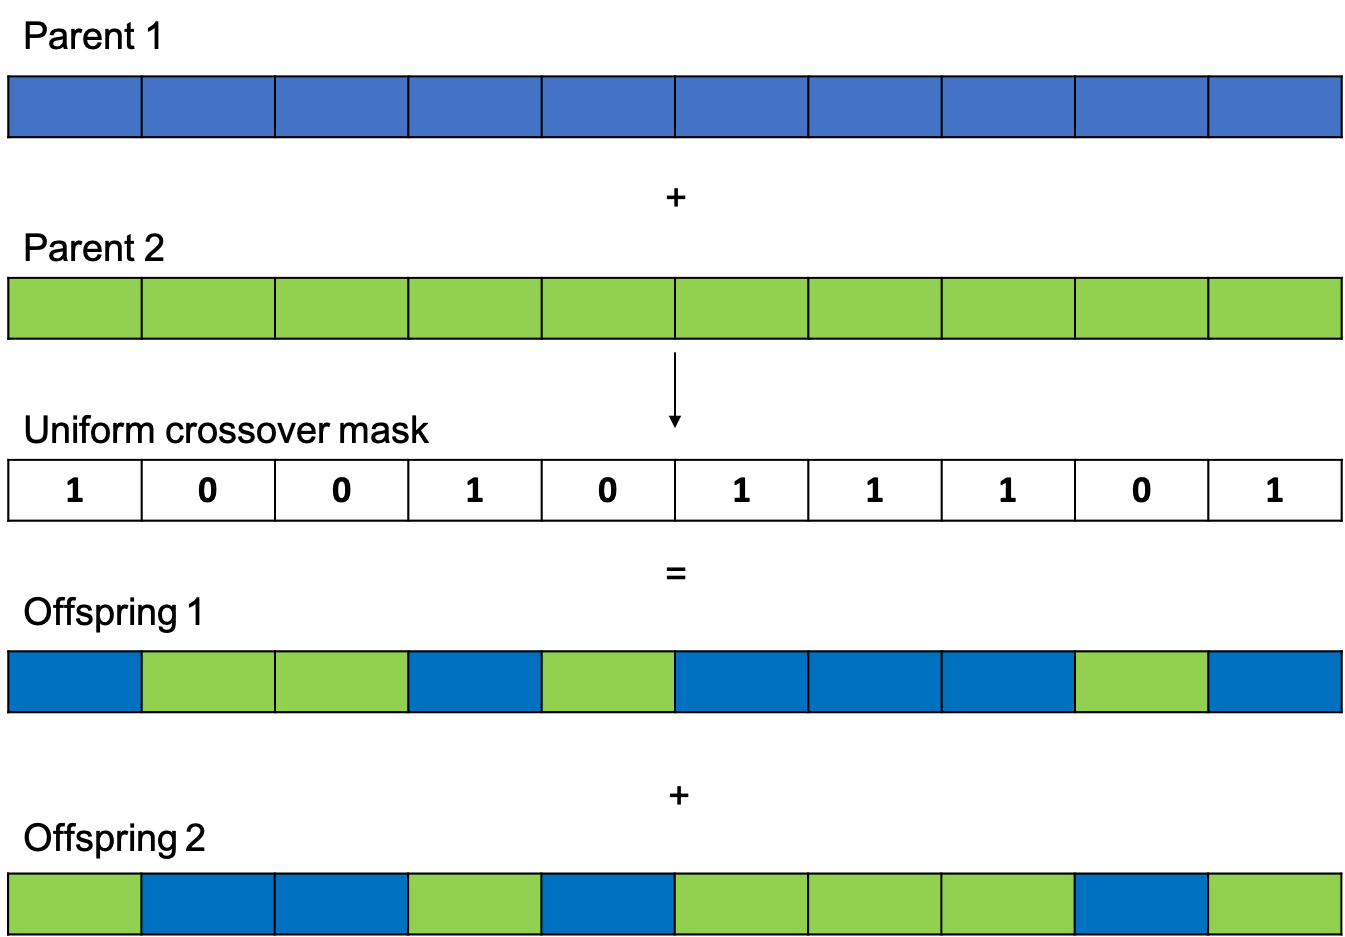
\includegraphics[width=0.8\textwidth]{images/uniform_crossover.pdf}
      \caption{An illustration of the uniform \index{crossover}crossover operator as it applies to sexual recombination, resulting in two new offspring.}
      \label{fig:heuristics:mh:ga:uniform_crossover}
\end{figure}


\begin{algorithm}[htb]
      \caption{The pseudo-code for the uniform \index{crossover}crossover operator as used by \acp{GA}.}
      \label{algo:heuristics:mh:ga:uniform_crossover}
      \begin{algorithmic}
            \State Initialise the mask, $m_{j}(t) = 0, \forall j = 1, \dots, J$;
            \For{$j = 1$ to $J$}
            \If{$U(0,1) \leq p_{x}$}
            \State $m_{j}(t) = 1$;
            \EndIf
            \EndFor
            \State
      \end{algorithmic}
\end{algorithm}


\subsubsection{Mutation}\label{sec:heuristics:mh:ga:mutation}

The \index{mutation}mutation operator is applied in order to introduce new genetic material into an existing entity~\cite{ref:engelbrecht:2007}. In doing so, diversity is added into the genetic characteristics of the population. Mutation is applied at a certain \index{mutation}mutation probability $p_{m}$, to each gene of the offspring $\boldsymbol{x}_{i}(t)$ to produce mutated offspring $\boldsymbol{x}'_{i}(t)$.~\citeauthor{ref:engelbrecht:2007}~\cite{ref:engelbrecht:2007} mentions that the \index{mutation}mutation probability, also referred to as the \index{mutation}mutation rate, is usually small such that $p_{m} \in [0,1]$ to ensure that good solutions are not distorted too much.

Similar to the \index{crossover}crossover operator, \index{mutation}mutation operators can be classified according to the representation scheme used. In the context of training
\acp{FFNN}, binary \index{crossover}crossover operators such as the \textit{uniform} \index{mutation}mutation operator can be used to generate a \index{mutation}mutation mask that specifies which genes are mutated. For the purposes of this dissertation, the application of the \index{mutation}mutation operator on $x_{ij}(t)$ results in a small update step for that gene such that $x'_{ij}(t) = x_{ij}(t) + v_{ij}(t)$. In this case, $v_{ij}(t)$ is sampled using \index{Glorot uniform sampling}Glorot uniform sampling within the bounds $(-limit, limit)$, as was presented in Chapter~\ref{chap:anns}. An adaptation of the uniform \index{mutation}mutation operator is provided in Algorithm~\ref{algo:heuristics:mh:ga:uniform_mutation} below.

\begin{algorithm}[htb]
      \caption{The pseudo-code for the uniform \index{mutation}mutation operator as used by \acp{GA}.}
      \label{algo:heuristics:mh:ga:uniform_mutation}
      \begin{algorithmic}
            \For{$i = 1$ to $N$}
            \For{$j = 1$ to $J$}
            \If{$U(0,1) \leq p_{m}$}
            \State Sample update step $v_{ij}(t) \sim U(-limit, limit)$
            \State $x'_{ij}(t) = x_{ij}(t) + v_{ij}(t)$;
            \EndIf
            \EndFor
            \EndFor
            \State
      \end{algorithmic}
\end{algorithm}

An illustration of the adapted uniform \index{mutation}mutation operator is presented in Figure~\ref{fig:heuristics:mh:ga:uniform_mutation} below.

\begin{figure}[htbp]
      \centering
      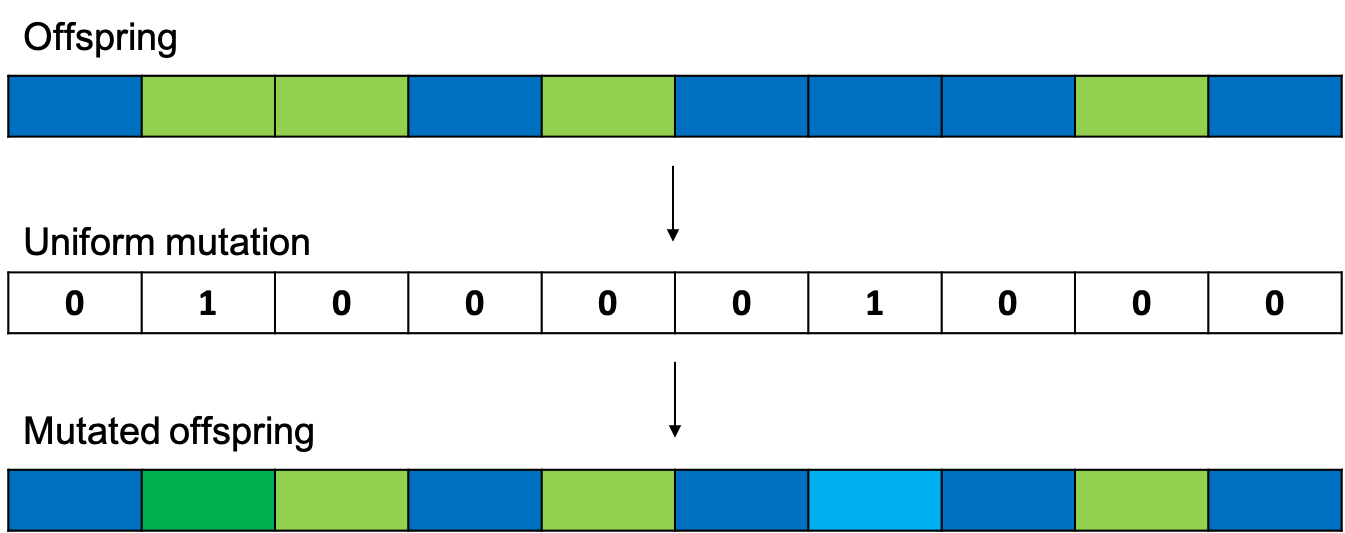
\includegraphics[width=0.8\textwidth]{images/uniform_mutation.pdf}
      \caption{An illustration of the adapted uniform \index{mutation}mutation operator as it applies to mutated offspring.}
      \label{fig:heuristics:mh:ga:uniform_mutation}
\end{figure}

\subsubsection{Selection}
\label{sec:heuristics:mh:ga:selection}

Selection is a widely used concept in all \acp{EA} and models survival of the fittest in the evolutionary context. The main idea behind the selection operator is to emphasise better solutions~\cite{ref:engelbrecht:2007}. Selection is applied in two of the main steps of \acp{EA}. These include:

\begin{itemize}
      \item \textbf{Selection of the new population:} A new population of candidate solutions are selected at the end of each generation to serve as the population for the next generation. The new population can be selected from both the parents and offspring. The selection operator is thus responsible for ensuring that good entities survive to the next generation.

      \item \textbf{Reproduction:} Offspring is created through the \index{crossover}crossover and/or the \index{mutation}mutation operators. In terms of \index{crossover}crossover, good solutions should have a high probability of reproducing to ensure that offspring contain genetic material of the best entities. In terms of \index{mutation}mutation, selection mechanisms should focus on weaker entities. By mutating weak entities, the hope is to introduce better traits, increasing their chance to survive.
\end{itemize}

\citeauthor{ref:engelbrecht:2007}~\cite{ref:engelbrecht:2007} mentions that selection operators are characterised by their \textit{selective pressure}. Selective pressure is defined as the speed at which the best entity's solution will occupy the entire population by repeated application of the selection operator alone~\cite{ref:back:1994}. A selection operator with a high selective pressure rapidly decreases the diversity in the population, possibly leading to premature convergence. A high selective pressure limits the exploration abilities of the population. Selection operators should maintain a balance between exploration and exploitation.

Various selection mechanisms have been proposed. For the purposes of this dissertation, focus is put on the following selection mechanisms and concepts.

\begin{itemize}
      \item \textbf{Tournament Selection:} Tournament selection selects a group of $N_{t}$ entities randomly from the population such that $N_{t} < N$, where $N$ is the population size. The performance of the selected $N_{t}$ entities are then compared and the best entities from this group are selected and returned by the operator. It should be mentioned that for sexual \index{crossover}crossover of two parents, tournament selection is applied twice, first for the first parent and then again for the second parent.~\citeauthor{ref:engelbrecht:2007}~\cite{ref:engelbrecht:2007} mentions that tournament selection prevents the best entities from dominating, provided that $N_{t}$ is not too large. This results in a lower selective pressure. If $N_{t}$ is too small, the chances that bad entities will be selected increase.

      \item \textbf{Rank-based Selection:} Rank-based selection uses the rank-ordered fitness values to determine the probability of selection and not the absolute fitness value.~\citeauthor{ref:engelbrecht:2007}~\cite{ref:engelbrecht:2007} mentions that the advantage of this approach is that the best entities will not dominate the selection process. Non-deterministic linear sampling selects an entity $\boldsymbol{x}_{i}(t)$ such that $i \sim U(0, U(0, N - 1))$. Importantly, in the context of a minimisation problem, entities are first sorted in decreasing order of fitness value, assuming that the best heuristic is then contained at index 0, while the worst entity is contained at index $N - 1$.

      \item \textbf{Elitism:} \index{elitism}Elitism refers to the process of ensuring that the best entities from the current population survive to the next generation. The best entities are simply passed on to the next generation without \index{mutation}mutation. The more entities that survive to the next generation, the lower the diversity of the new population.
\end{itemize}


\section{Summary}
\label{sec:heuristics:summary}

This chapter provided detailed background information on \index{heuristic}heuristics. Different heuristics were presented that have been shown to be able to train \acp{FFNN}. Two main groups of \index{heuristic}heuristics where presented and discussed in detail. These include gradient-based \index{heuristic}heuristics and \acfp{MH}. A number of different variants for each group have been presented and was discussed in detail.
